\documentclass[11pt]{article}

\usepackage[final]{acl}

% Standard package includes
\usepackage{times}
\usepackage{latexsym}
\usepackage[T1]{fontenc}
\usepackage[utf8]{inputenc}
\usepackage{microtype}
\usepackage{graphicx}
\usepackage{booktabs}
\usepackage{array}
\usepackage{url}
\usepackage{enumitem}
\usepackage{amssymb}
% Allow slight extra stretch to avoid underfull hboxes in narrow ACL columns
\emergencystretch=2em

\title{Counterfactual Student Intervention Dashboard:\\Prototype Report}

\author{Yiming Xiao \\
  Texas A\&M University \\
  UIN: 835009298\\
  \texttt{yxiao@tamu.edu} \\\And
  Yi-Hsin Chiang \\
  Texas A\&M University \\
  UIN:137001082 \\
  \texttt{yihsin.chiang@tamu.edu} \\}
\hyphenpenalty=10000
\begin{document}
{\makeatletter\acl@finalcopytrue
  \maketitle
}

\begin{abstract}
This report presents the design, implementation, and current status of \textit{Counterfactual Visual Analytics for Targeted Student Interventions}, an interactive visualization system that combines multiple linear regression with bootstrapped confidence intervals and real-time counterfactual ``what-if'' exploration. Building on a survey of five educators (two professors and three teaching assistants), we derive four design requirements and map them to five implemented visualization features. The working prototype, built with D3.js, fits a linear regression model ($R^2 = 0.727$) with 220 bootstrap resamples to produce predicted score distributions. Instructors can select at-risk students, manipulate actionable variables via interactive sliders and dropdowns, and instantly compare a student's baseline trajectory against an intervened scenario. All core functions are operational, and this report documents the system architecture, interface design, and code inventory.
\end{abstract}

% -----------------------------------------------------------------------
\section{Introduction}
% -----------------------------------------------------------------------

Early identification of at-risk students and timely intervention are two of the most effective levers available to higher-education institutions for improving retention and academic outcomes. Yet the dashboards most commonly used by instructors today are fundamentally backward-looking. They surface grades, attendance records, and class averages after the fact, giving educators a clear picture of \textit{what happened} but no systematic way to reason about \textit{what to do next}. A professor who notices a student trending toward failure is left to rely on intuition or informal heuristics when deciding whether to recommend additional tutoring, encourage better attendance, or suggest improved sleep habits.

This gap between descriptive reporting and actionable guidance is the core problem we address. We present a causal-predictive visual analytics system that moves beyond historical summaries to support forward-looking, evidence-based decision making. The key idea is counterfactual reasoning: given a student's current profile, the system asks ``What would the predicted outcome be \textit{if} we changed variable $X$ by a certain amount?'' and renders the answer as an immediately interpretable visual comparison.

Concretely, we fit a multiple linear regression model on a student performance dataset containing 20 features per student. The predictions are accompanied by confidence intervals derived from 220 bootstrap resamples so that advisors can see not just a point estimate but the uncertainty around it. An interactive intervention panel exposes sliders for actionable variables. Moving a slider instantly redraws a predicted score distribution on top of the student's baseline, making the expected benefit of each intervention immediately visible.

This report makes three contributions: (1)~a design requirement analysis grounded in a survey of five educators, (2)~a working interactive prototype that implements counterfactual visual analytics with uncertainty visualization, and (3)~a systematic mapping from design requirements to implemented features.

% -----------------------------------------------------------------------
\section{Related Work}
\label{sec:related}
% -----------------------------------------------------------------------

\paragraph{Learning analytics and dashboards.}
The field of learning analytics has produced a wide range of tools aimed at monitoring and improving student outcomes \cite{siemens2013learning}. Most deployed dashboards, however, remain in the descriptive analytics tier: they aggregate log data, attendance, and grade records into visualizations that help instructors see where students stand, but they do not prescribe interventions \cite{papamitsiou2014learning}. Our work is motivated by the observation that bridging descriptive and prescriptive analytics requires an explicit model of how changing behavior leads to changed outcomes.

\paragraph{Prediction models for student performance.}
Machine learning models for predicting student success have been extensively studied \cite{romero2020educational}. \citet{asselman2023} demonstrate that gradient-boosted models such as XGBoost achieve strong predictive accuracy, and \citet{khalaf2025} show that ensemble regressors further improve performance. A recurring theme in this literature is that accuracy alone is insufficient: without interpretability, educators cannot act on model outputs. This motivates our choice of multiple linear regression, whose coefficients are directly interpretable as marginal effects of each feature on the predicted exam score.

\paragraph{Counterfactual explanations in education.}
Counterfactual explanations have attracted growing interest in educational data mining \cite{bunay2026}. \citet{tsiakmaki2021} show that interpretable counterfactual explanations can identify critical factors for student success and support personalized educational strategies. \citet{afrin2023} apply Diverse Counterfactual Explanations (DiCE) to show that changes in study behavior can shift students from failing to passing, a finding validated through a user study with educators. \citet{susnjak2022} demonstrate the use of predictive and counterfactual learning analytics panels to estimate academic success. A recent systematic review~\cite{bunay2026} finds that counterfactual methods are increasingly applied to student dropout and retention, but no consensus exists on which generation method is most suitable. Our system extends this line of work by embedding counterfactual generation inside an interactive visual analytics interface with uncertainty visualization.

\paragraph{Visual analytics for dropout and at-risk students.}
Several systems have explicitly targeted at-risk student identification through visualization. \citet{sdavis2022} introduce SDA-Vis, a system that supports counterfactual exploration of student dropout dynamics across academic, social, and economic variables. \citet{zhang2023} combine a CNN-LSTM model with counterfactual explanations to visually analyze dropout behavior patterns in online learning environments, quantifying the impact of behavioral changes on dropout probability. Both systems demonstrate the value of embedding counterfactual reasoning inside a visual interface, which is the approach we pursue for the general exam-score prediction setting.

% -----------------------------------------------------------------------
\section{Design Requirement Analysis}
\label{sec:requirements}
% -----------------------------------------------------------------------

\subsection{Survey Methodology}

To ground the system design in the needs of real educators, we conducted a structured online survey using Google Forms. Five participants took part: two university professors and three teaching assistants, all with direct experience advising or monitoring student progress. The questionnaire consisted of five multiple-choice questions covering: (1)~what information educators look at first when a student is struggling, (2)~which factors feel most actionable, (3)~which system outputs would be most useful for decision-making, (4)~which interface elements would feel easiest to use, and (5)~what factors matter most for trusting such a tool.

\subsection{Survey Results}

\paragraph{Information priorities (Q1).} When noticing a struggling student, respondents first look at homework and assignment completion (40\%), exam and quiz grades (40\%), and attendance (20\%). No respondent selected participation/engagement or previous academic performance as their first source.

\paragraph{Actionable factors (Q2).} All five respondents (100\%) identified tutoring and office hours as actionable. Study time and study habits were selected by 80\%, as was access to learning resources. Attendance was considered actionable by 60\%, and sleep/personal routines by 40\%.

\paragraph{Useful outputs (Q3).} The most valued outputs were comparison between baseline and intervention scenario (60\%) and comparison with class averages (60\%). Probability of falling below a passing threshold was selected by 40\%. Notably, neither ``predicted exam score after intervention'' nor ``ranked list of most impactful interventions'' received any votes as a standalone output.

\paragraph{Interface preferences (Q4).} A chart showing before/after prediction changes was rated easiest to use by 80\% of respondents, tied with sliders for numeric variables (80\%). Dropdowns for categorical variables, preset intervention buttons, and summary cards with recommended next steps were each selected by 40\%.

\paragraph{Trust factors (Q5).} Consistency with the educator's own experience was the top trust factor (80\%). Simple and interpretable explanations (60\%), clear uncertainty/confidence ranges (60\%), and easy comparison between multiple interventions (60\%) followed closely. Only 20\% selected ``only showing realistic/actionable variables.''

\subsection{Design Requirements}

Based on the survey results, the literature review (Section~\ref{sec:related}), and the actionability taxonomy of the dataset features, we derive four design requirements:

\begin{description}[leftmargin=1cm, style=nextline]
  \item[\textbf{D1}] \textbf{Quickly identify at-risk students and prioritize attention.} Educators' first instinct is to check grades and attendance (Q1). The system must surface struggling students immediately without requiring manual data lookups.

  \item[\textbf{D2}] \textbf{Compare baseline prediction against intervention scenarios in real time.} The most valued output is a baseline-vs.-intervention comparison (Q3, 60\%), and the preferred visualization is a before/after prediction chart (Q4, 80\%). The system must let users see the predicted shift as they adjust variables.

  \item[\textbf{D3}] \textbf{Provide interpretable, actionable guidance for next steps.} All respondents consider tutoring actionable (Q2, 100\%), and 80\% want study time and resource access to be adjustable. Trust depends on simple, interpretable explanations (Q5, 60\%) and consistency with experience (Q5, 80\%). The model must be transparent and the interface must highlight which levers yield the largest gains.

  \item[\textbf{D4}] \textbf{Communicate prediction uncertainty and contextual grounding.} Respondents value clear confidence ranges (Q5, 60\%) and comparison with class averages (Q3, 60\%). The system must show not just point estimates but distributional information and contextual benchmarks.
\end{description}

% -----------------------------------------------------------------------
\section{Dataset and System Overview}
\label{sec:system}
% -----------------------------------------------------------------------

\subsection{Dataset}

We use the \textit{Student Academic Performance Dataset} by Ayesha Siddiqa, publicly available on Kaggle. The dataset records 20 features per student across 6{,}607 records, with the final exam score as the target variable. Table~\ref{tab:features} summarizes the features by category, illustrating their data types and counterfactual actionability.

\begingroup
\renewcommand{\arraystretch}{1.5}
\begin{table*}[t]
\centering
\small
\begin{tabular}{p{3.0cm} p{6cm} p{1.5cm} p{3.5cm}}
\toprule
\textbf{Category} & \textbf{Example Variables} & \textbf{Type} & \textbf{Actionability} \\
\midrule
Academic History & Previous\_Scores, Exam\_Score & Numeric & Immutable (baseline) \\
Student Behavior & Hours\_Studied, Attendance & Numeric & High (direct) \\
Lifestyle \& Habits & Sleep\_Hours, Extracurricular & Num./Cat. & Moderate (counseling) \\
Environment \& Support & Tutoring\_Sessions, Parental\_Involvement & Cat. & Partial (resources) \\
\bottomrule
\end{tabular}
\caption{Feature categories, example variables, data types, and counterfactual actionability.}
\label{tab:features}
\end{table*}
\endgroup

Figure~\ref{fig:corr} shows the Pearson correlation matrix for the main numeric features. The strongest correlates of Exam\_Score are Attendance ($r = 0.58$) and Hours\_Studied ($r = 0.45$), followed by Previous\_Scores, Access\_to\_Resources, and Tutoring\_Sessions. The low inter-feature correlations indicate that multicollinearity is not a serious concern for the regression model.

\begin{figure}[h]
  \centering
  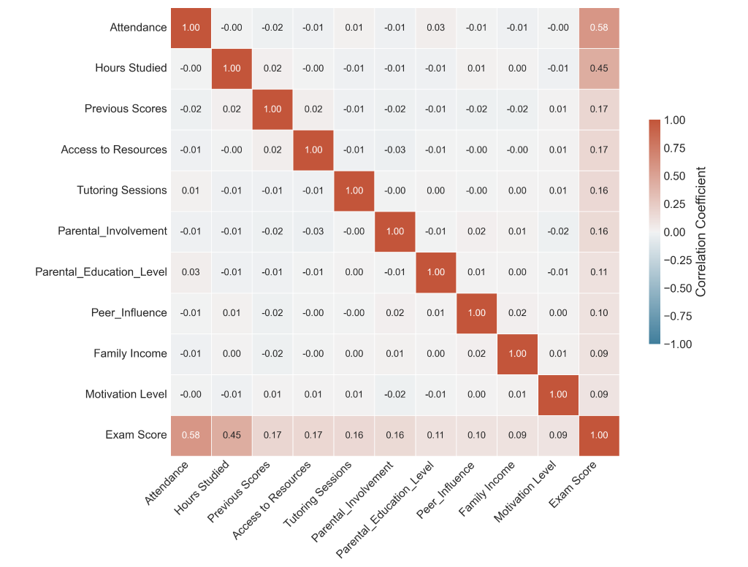
\includegraphics[width=\columnwidth]{corr.png}
  \caption{Pearson correlation matrix for numeric student features.}
  \label{fig:corr}
\end{figure}

\subsection{Statistical Model}

We fit a multiple linear regression model of the form
\[
  \hat{y} = \beta_0 + \sum_{j=1}^{p} \beta_j x_j,
\]
where $\hat{y}$ is the predicted exam score and $x_1, \ldots, x_p$ are the 20 student features (with categorical variables ordinally encoded). The model is trained using ordinary least squares with a small ridge penalty ($\lambda = 10^{-6}$) for numerical stability. The fitted model achieves $R^2 = 0.727$ with a residual standard deviation of 2.03 points.

We apply the bootstrap ($B = 220$ resamples) to obtain confidence intervals around each coefficient and each individual prediction. For a given student profile, each of the 220 bootstrap models produces an independent prediction, yielding a predicted score \textit{distribution} rather than a point estimate. This distribution is visualized as a kernel density estimate (KDE) curve using a Gaussian kernel with Silverman's bandwidth rule.

A key design choice is to favor a transparent model over a more complex black-box predictor. Each coefficient $\beta_j$ is directly interpretable as ``an additional tutoring session per week is associated with $+\beta_j$ exam-score points.'' This transparency is essential for user trust (\textbf{D3}) and allows advisors to reason about the practical meaning of each slider adjustment.

\subsection{Data Pipeline}

The data pipeline is implemented in Python (${\sim}336$ lines). It performs the following steps:
\begin{enumerate}
  \item Load the raw CSV (6{,}607 rows) and impute missing values (mode for categorical, median for numeric).
  \item Ordinally encode categorical features (e.g., Low$=0$, Medium$=1$, High$=2$).
  \item Fit the linear regression model and generate 220 bootstrap resamples.
  \item Select 18 focus students (12 critical with score $<60$, 6 borderline with score 60--64).
  \item Compute top feature correlations, a 500-student cohort scatter sample, and preset intervention bundles.
  \item Export all data as a single JavaScript file (${\sim}270$\,KB) consumed directly by the frontend.
\end{enumerate}

\subsection{System Workflow}

The system supports a six-step advising workflow:

\begin{enumerate}
  \item \textbf{Select a student} from the Focus Students panel (left sidebar).
  \item \textbf{Review Score Summary Tiles} showing the actual score, baseline prediction, scenario prediction, and intervention lift.
  \item \textbf{Inspect the Predicted Score Distribution}: dual kernel density curves (baseline in amber, scenario in teal) with a shaded fail zone below score 60.
  \item \textbf{Adjust interventions} using preset buttons (Attendance Recovery, Tutoring Boost, Study Plan) or by manually tuning sliders and dropdowns for individual variables.
  \item \textbf{Review Best Next Levers}: a ranked list of the top single-step interventions sorted by predicted score gain, with one-click apply buttons.
  \item \textbf{Check contextual views}: the cohort scatter plot, top correlations bar chart, and immutable factors grid to ground the prediction in broader context.
\end{enumerate}

% -----------------------------------------------------------------------
\section{Interface Design and Features}
\label{sec:interface}
% -----------------------------------------------------------------------

The prototype is a single-page web application built with D3.js \cite{bostock2011}. It requires no server or build step---opening \texttt{index.html} in a browser launches the full dashboard. This section describes each visualization feature and maps it to the design requirements from Section~\ref{sec:requirements}.

\subsection{Feature Summary}

Table~\ref{tab:feature-mapping} provides an overview of the five main features and their mapping to design requirements.

\begin{table*}[t]
\centering
\small
\renewcommand{\arraystretch}{1.3}
\begin{tabular}{c p{4cm} p{6cm} c c c c}
\toprule
\textbf{ID} & \textbf{Feature} & \textbf{Description} & \textbf{D1} & \textbf{D2} & \textbf{D3} & \textbf{D4} \\
\midrule
F1 & Focus Students Panel & Scrollable list of 18 at-risk students with actual/predicted scores and risk-band badges. & $\checkmark$ & & & \\
F2 & Predicted Score Distribution & Dual KDE density curves (baseline vs.\ scenario) with fail zone, rug plots, Score Summary Tiles, and Scenario Feedback. & & $\checkmark$ & & $\checkmark$ \\
F3 & Best Next Levers & Ranked single-step interventions by predicted gain, with one-click apply and Model Signals (coefficients with CIs). & & & $\checkmark$ & \\
F4 & Editable Intervention Controls & Sliders for numeric variables, dropdowns for categorical, presets, and Reset. Shows baseline vs.\ current value. & & $\checkmark$ & $\checkmark$ & \\
F5 & Context \& Correlation Views & Immutable factors grid, cohort scatter plot, and top correlations bar chart. & & & & $\checkmark$ \\
\bottomrule
\end{tabular}
\caption{Feature-to-Requirement mapping. Each feature (F1--F5) addresses one or more design requirements (D1--D4).}
\label{tab:feature-mapping}
\end{table*}

\subsection{F1: Focus Students Panel}

The left sidebar displays 18 pre-selected focus students, chosen by the data pipeline as the lowest-scoring and borderline cases in the dataset. Each student card shows the student ID, actual exam score, model-predicted baseline score, and a color-coded risk badge:
\begin{itemize}
  \item \textbf{Critical} (red): predicted score $< 60$
  \item \textbf{Watch} (amber): predicted score 60--67
  \item \textbf{Stable} (teal): predicted score 67--75
  \item \textbf{Strong} (navy): predicted score $> 75$
\end{itemize}
Clicking a student card loads their full profile into all other panels. This feature directly addresses \textbf{D1} by letting advisors quickly triage who needs attention.

\subsection{F2: Predicted Score Distribution}

The central visualization is a predicted score distribution chart rendered as an SVG with D3.js (860$\times$430\,px). It displays two overlapping kernel density curves:

\begin{itemize}
  \item \textbf{Baseline (amber)}: the predicted distribution given the student's current feature values.
  \item \textbf{Scenario (teal)}: the predicted distribution under the user's proposed intervention.
\end{itemize}

The chart includes a shaded red fail zone (score $< 60$), a dashed threshold line at 60, vertical dashed markers for the baseline mean, scenario mean, and actual score, and rug plots at the bottom showing each of the 220 bootstrap prediction values. A legend displays the baseline and scenario means.

Above the chart, four \textbf{Score Summary Tiles} show: (1)~the actual exam score with observed risk band and passing threshold, (2)~baseline expected score with 90\% confidence interval and failure risk percentage, (3)~scenario expected score with 90\% CI and failure risk, and (4)~the intervention lift (score delta, failure risk change, and number of modified levers).

A \textbf{Scenario Feedback} box below the tiles displays contextual messages such as ``Scenario is at baseline,'' ``Has $N$ edited levers,'' or ``Applied recommendation: Tutoring sessions.''

This feature addresses \textbf{D2} (real-time baseline-vs.-scenario comparison) and \textbf{D4} (uncertainty visualization via the density curves and confidence intervals).

% TODO: Add screenshot of the Predicted Score Distribution panel
\begin{figure*}[h]
  \centering
  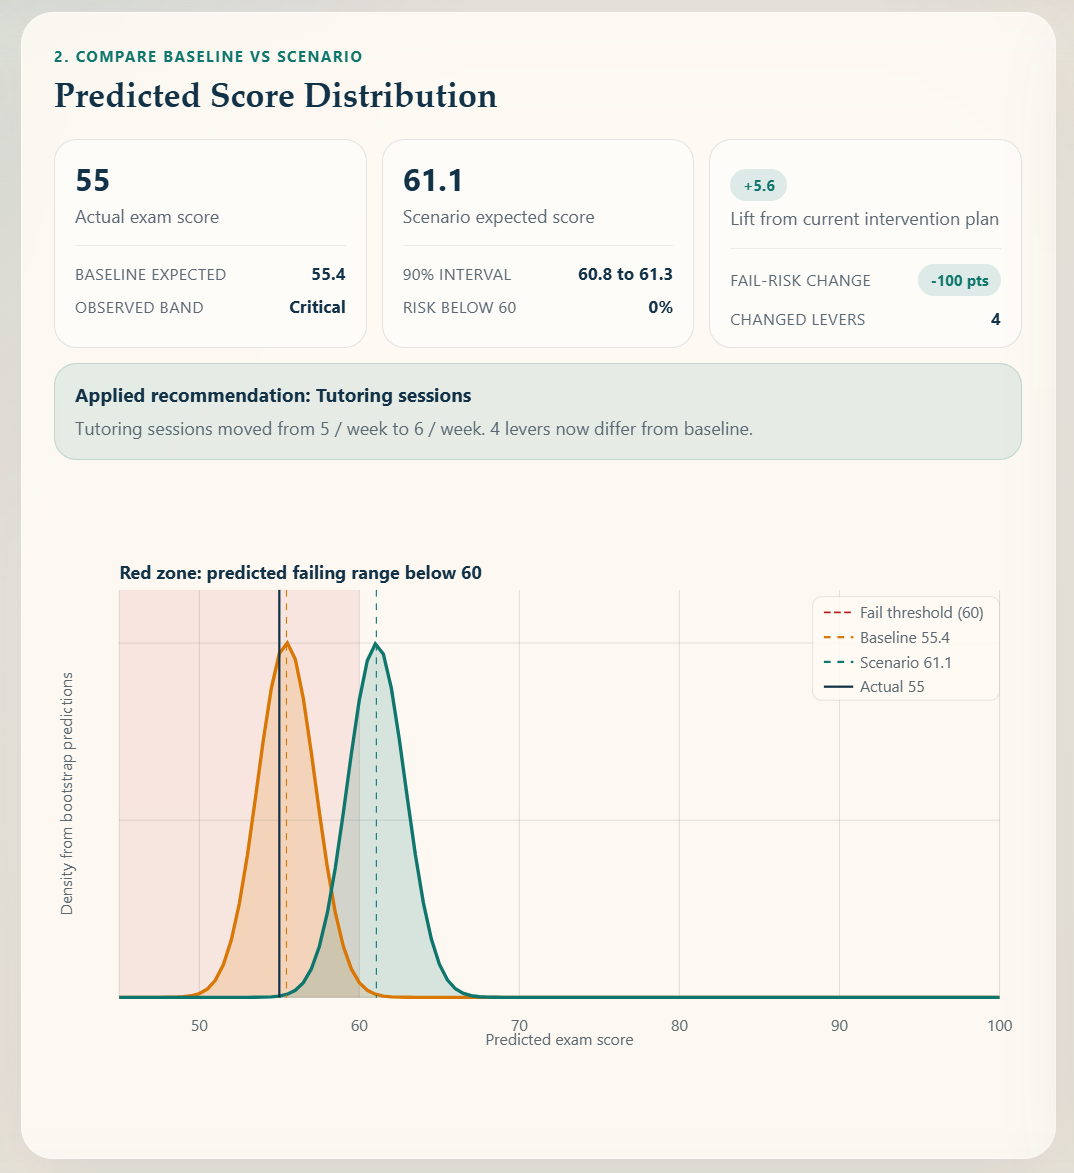
\includegraphics[width=1.5\columnwidth]{dash.png}
  \caption{Screenshot of the Predicted Score Distribution panel showing baseline (amber) and scenario (teal) density curves for Student 1102 after applying three interventions. The fail zone (score $< 60$) is shaded in red.}
  \label{fig:dashboard}
\end{figure*}

\subsection{F3: Best Next Levers (Decision Support)}

The right sidebar provides a \textbf{Best Next Levers} panel that ranks up to five single-step interventions by predicted score gain. For each recommended lever, the panel shows the feature name, the suggested next value, and the expected point increase (e.g., ``Access to resources $\rightarrow$ Medium, $+1.0$ pts''). An ``Apply This Lever'' button lets the advisor accept the recommendation with one click, immediately updating the scenario prediction.

Below the recommendations, a \textbf{Model Signals} sub-panel displays the top five regression coefficients with their bootstrap confidence intervals, color-coded green (positive) or red (negative). This transparency lets advisors verify that the model's recommendations align with their domain knowledge, directly supporting \textbf{D3}.

\subsection{F4: Editable Intervention Controls}

The Intervention Controls panel exposes all actionable variables organized in a three-column grid. Controls are differentiated by actionability level:

\begin{itemize}
  \item \textbf{Directly actionable} (sliders): Attendance (60--100\%), Hours~Studied (1--44\,hrs), Tutoring~Sessions (0--8/week).
  \item \textbf{Counseling or resource levers} (sliders and dropdowns): Sleep Hours, Physical Activity, Motivation Level, Access to Resources, Extracurricular Activities, Internet Access, and Parental Involvement.
\end{itemize}

Each control card displays the current value, an ``Edited'' or ``Baseline'' tag, and the original baseline value for reference. Moving a slider or changing a dropdown instantly redraws the scenario density curve in F2 without requiring a button press.

Four \textbf{preset buttons} provide one-click intervention bundles:
\begin{itemize}
  \item \textbf{Attendance Recovery}: $+6$\% attendance, $+1$\,hr sleep.
  \item \textbf{Tutoring Boost}: $+2$ tutoring sessions/wk, $+1$ resource level.
  \item \textbf{Study Plan}: $+4$ study hours, $+1$ motivation level, add extracurriculars.
  \item \textbf{Reset to Baseline}: reverts all changes to the original student profile.
\end{itemize}

This feature addresses \textbf{D2} (real-time scenario exploration) and \textbf{D3} (actionable guidance through clearly labeled controls).

% TODO: Add screenshot of the Intervention Controls panel
\begin{figure*}[h]
  \centering
  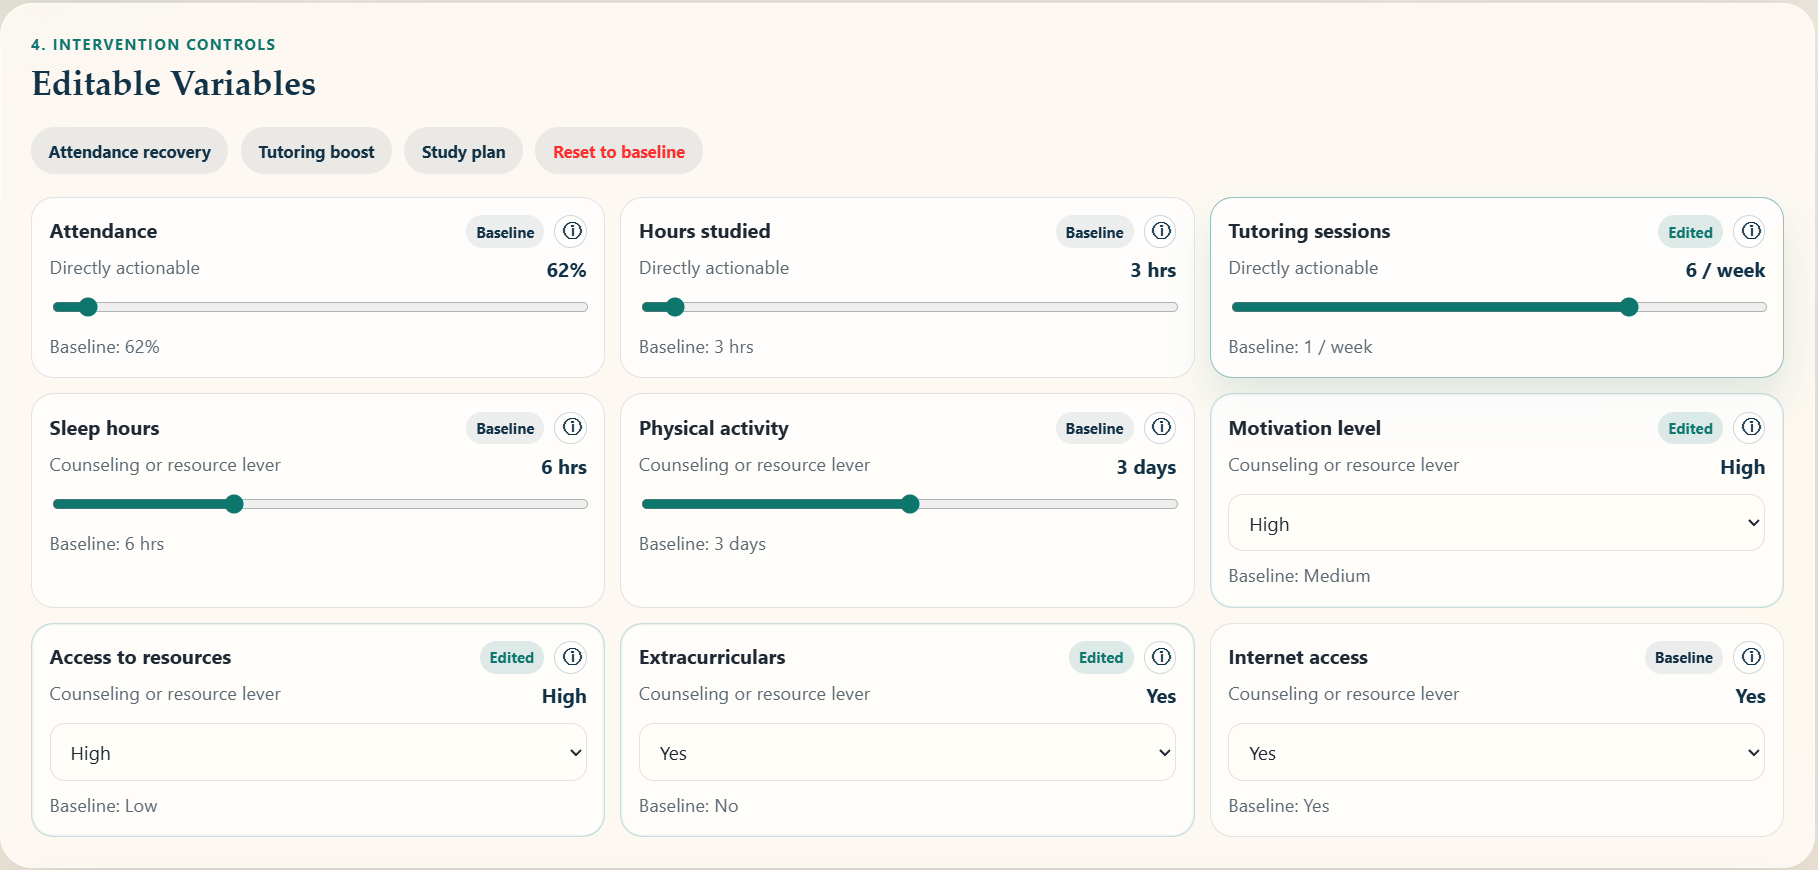
\includegraphics[width=2\columnwidth]{control.png}
  \caption{The Intervention Controls panel showing sliders for directly actionable variables, dropdowns for categorical levers, and preset intervention buttons.}
  \label{fig:controls}
\end{figure*}

\subsection{F5: Context and Correlation Views}

Three contextual panels ground the prediction in broader context:

\paragraph{Immutable Structural Factors.} A three-column card grid displays non-actionable student attributes: Previous Score, Family Income, Teacher Quality, Peer Influence, Parental Education Level, Distance from Home, Gender, School Type, Learning Disabilities, and Parental Involvement. These are shown for context but cannot be edited, reinforcing the distinction between actionable and immutable variables.

\paragraph{Cohort Overview Scatter Plot.} A D3.js scatter plot (560$\times$300\,px) shows Attendance vs.\ Exam Score for a 500-student sample, colored by Parental Involvement level (Low in red, Medium in amber, High in teal). The currently selected student is highlighted with a navy crosshair, allowing the advisor to see where the student falls relative to the cohort.

\paragraph{Top Correlations Bar Chart.} A horizontal bar chart (560$\times$300\,px) ranks the 10 features most correlated with Exam Score by Pearson $r$, color-coded green (positive) or red (negative). The top correlates are Attendance ($r = 0.581$) and Hours Studied ($r = 0.445$).

These views address \textbf{D4} by providing contextual grounding and class-average comparisons that respondents valued (Q3, 60\%).

% -----------------------------------------------------------------------
\section{Implementation}
\label{sec:implementation}
% -----------------------------------------------------------------------

\subsection{Code Architecture}

The system follows a three-layer architecture with no runtime server:

\begin{enumerate}
  \item \textbf{Data pipeline} (Python, ${\sim}336$ lines): loads the raw CSV, fits the regression model, generates 220 bootstrap resamples, selects focus students, and exports all data as a single JavaScript file.
  \item \textbf{Pre-computed data layer} (${\sim}270$\,KB): a generated JavaScript file that populates a global object with student profiles, bootstrap models, feature definitions, encoding maps, and preset intervention bundles.
  \item \textbf{Frontend} (${\sim}1{,}100$ lines of JS): A single-page D3.js application (\texttt{app.js}, \texttt{index.html}, \texttt{styles.css}) that renders all visualizations, manages state, and handles user interactions.
\end{enumerate}

The only external dependency is D3.js~v7, vendored locally. The prototype runs by opening \texttt{index.html} in any modern browser.

\subsection{Function Inventory}

Tables~\ref{tab:frontend-functions} and \ref{tab:backend-functions} list the key functions in the frontend and backend, respectively, along with their purpose and current status. All functions are fully operational.

\begin{table*}[t]
\centering
\small
\renewcommand{\arraystretch}{1.2}
\begin{tabular}{l p{8cm} l}
\toprule
\textbf{Function} & \textbf{Purpose} & \textbf{Status} \\
\midrule
\texttt{predictWithModel} & Compute predicted score from feature values using one bootstrap model's coefficients & Working \\
\texttt{getPredictionSamples} & Run all 220 bootstrap models to produce a prediction distribution & Working \\
\texttt{buildDensity} & Kernel density estimation with Silverman bandwidth and Gaussian kernel (440 grid points) & Working \\
\texttt{buildRecommendations} & Rank single-step interventions by predicted score gain & Working \\
\texttt{renderPredictionChart} & D3.js dual-density chart with fail zone, rug plots, markers, and legend & Working \\
\texttt{renderStudentList} & Student selection cards with risk-band badges & Working \\
\texttt{renderControls} & Slider and dropdown controls with baseline comparison & Working \\
\texttt{renderPresets} & Preset intervention buttons (Attendance Recovery, Tutoring Boost, Study Plan) & Working \\
\texttt{renderScatterChart} & D3.js cohort scatter plot with selected-student highlight & Working \\
\texttt{renderCorrelationChart} & D3.js horizontal bar chart of top feature correlations & Working \\
\texttt{renderRecommendations} & Decision support cards with ``Apply This Lever'' buttons & Working \\
\texttt{renderScoreSummary} & Four Score Summary Tiles (actual, baseline, scenario, lift) & Working \\
\texttt{renderContext} & Immutable Structural Factors grid & Working \\
\texttt{renderAll} & Orchestrator that calls all render functions on state change & Working \\
\bottomrule
\end{tabular}
\caption{Frontend function inventory (\texttt{prototype/app.js}, $\sim$1{,}100 lines). All 14 functions are working.}
\label{tab:frontend-functions}
\end{table*}

\begin{table*}[t]
\centering
\small
\renewcommand{\arraystretch}{1.2}
\begin{tabular}{l p{6cm} l}
\toprule
\textbf{Function} & \textbf{Purpose} & \textbf{Status} \\
\midrule
\texttt{fit\_linear\_model} & OLS regression with ridge penalty ($10^{-6}$) & Working \\
\texttt{build\_bootstrap\_models} & Generate 220 bootstrap resamples for uncertainty quantification & Working \\
\texttt{build\_student\_cards} & Select 18 focus students (lowest-scoring and borderline cases) & Working \\
\texttt{build\_top\_correlations} & Rank features by Pearson correlation with exam score & Working \\
\texttt{build\_cohort\_scatter} & Sample 500 students for the cohort overview scatter plot & Working \\
\bottomrule
\end{tabular}
\caption{Backend function inventory (\texttt{build\_prototype\_data.py}, ${\sim}336$ lines of Python). All 5 functions are working.}
\label{tab:backend-functions}
\end{table*}

In total, 19 out of 19 key functions (100\%) are fully operational. The prototype supports the complete advising workflow described in Section~\ref{sec:system}.

% -----------------------------------------------------------------------
\section{Evaluation Plan}
\label{sec:evaluation}
% -----------------------------------------------------------------------

We will conduct a \textbf{controlled usability study} comparing two conditions: a \textbf{baseline} in which participants use a standard spreadsheet (Excel) containing the student dataset with no model outputs, and a \textbf{system} condition in which participants use the interactive dashboard. We will measure two primary outcomes:

\begin{enumerate}
  \item \textbf{Time-to-Decision:} elapsed time from task start to committing to an intervention plan, measured via stopwatch.
  \item \textbf{Confidence Level:} self-reported 1--10 Likert scale asking ``How confident are you in your intervention plan?''.
\end{enumerate}

Secondary measures include the number and quality of distinct interventions proposed, and qualitative feedback from a brief post-task interview.

The preliminary survey results reported in Section~\ref{sec:requirements} provide early validation that the design requirements align with educator needs. The full evaluation study will test whether the implemented prototype delivers measurable improvements in decision speed and confidence.

% -----------------------------------------------------------------------
\bibliography{references}
\end{document}
